\documentclass[journal]{IEEEtran}
%
% If IEEEtran.cls has not been installed into the LaTeX system files,
% manually specify the path to it like:
% \documentclass[journal]{../sty/IEEEtran}





% Some very useful LaTeX packages include:
% (uncomment the ones you want to load)


% *** MISC UTILITY PACKAGES ***
%
%\usepackage{ifpdf}
% Heiko Oberdiek's ifpdf.sty is very useful if you need conditional
% compilation based on whether the output is pdf or dvi.
% usage:
% \ifpdf
%   % pdf code
% \else
%   % dvi code
% \fi
% The latest version of ifpdf.sty can be obtained from:
% http://www.ctan.org/pkg/ifpdf
% Also, note that IEEEtran.cls V1.7 and later provides a builtin
% \ifCLASSINFOpdf conditional that works the same way.
% When switching from latex to pdflatex and vice-versa, the compiler may
% have to be run twice to clear warning/error messages.

\usepackage{multirow}




% *** CITATION PACKAGES ***
%
\usepackage{cite}
% cite.sty was written by Donald Arseneau
% V1.6 and later of IEEEtran pre-defines the format of the cite.sty package
% \cite{} output to follow that of the IEEE. Loading the cite package will
% result in citation numbers being automatically sorted and properly
% "compressed/ranged". e.g., [1], [9], [2], [7], [5], [6] without using
% cite.sty will become [1], [2], [5]--[7], [9] using cite.sty. cite.sty's
% \cite will automatically add leading space, if needed. Use cite.sty's
% noadjust option (cite.sty V3.8 and later) if you want to turn this off
% such as if a citation ever needs to be enclosed in parenthesis.
% cite.sty is already installed on most LaTeX systems. Be sure and use
% version 5.0 (2009-03-20) and later if using hyperref.sty.
% The latest version can be obtained at:
% http://www.ctan.org/pkg/cite
% The documentation is contained in the cite.sty file itself.






% *** GRAPHICS RELATED PACKAGES ***
  \usepackage[pdftex]{graphicx}
  % declare the path(s) where your graphic files are
  \graphicspath{{./images/}}
  % and their extensions so you won't have to specify these with
  % every instance of \includegraphics
  \DeclareGraphicsExtensions{.pdf,.jpeg,.png}
% graphicx was written by David Carlisle and Sebastian Rahtz. It is
% required if you want graphics, photos, etc. graphicx.sty is already
% installed on most LaTeX systems. The latest version and documentation
% can be obtained at: 
% http://www.ctan.org/pkg/graphicx
% Another good source of documentation is "Using Imported Graphics in
% LaTeX2e" by Keith Reckdahl which can be found at:
% http://www.ctan.org/pkg/epslatex
%
% latex, and pdflatex in dvi mode, support graphics in encapsulated
% postscript (.eps) format. pdflatex in pdf mode supports graphics
% in .pdf, .jpeg, .png and .mps (metapost) formats. Users should ensure
% that all non-photo figures use a vector format (.eps, .pdf, .mps) and
% not a bitmapped formats (.jpeg, .png). The IEEE frowns on bitmapped formats
% which can result in "jaggedy"/blurry rendering of lines and letters as
% well as large increases in file sizes.
%
% You can find documentation about the pdfTeX application at:
% http://www.tug.org/applications/pdftex





% *** MATH PACKAGES ***
%
%\usepackage{amsmath}
% A popular package from the American Mathematical Society that provides
% many useful and powerful commands for dealing with mathematics.
%
% Note that the amsmath package sets \interdisplaylinepenalty to 10000
% thus preventing page breaks from occurring within multiline equations. Use:
%\interdisplaylinepenalty=2500
% after loading amsmath to restore such page breaks as IEEEtran.cls normally
% does. amsmath.sty is already installed on most LaTeX systems. The latest
% version and documentation can be obtained at:
% http://www.ctan.org/pkg/amsmath





% *** SPECIALIZED LIST PACKAGES ***
%
%\usepackage{algorithmic}
% algorithmic.sty was written by Peter Williams and Rogerio Brito.
% This package provides an algorithmic environment fo describing algorithms.
% You can use the algorithmic environment in-text or within a figure
% environment to provide for a floating algorithm. Do NOT use the algorithm
% floating environment provided by algorithm.sty (by the same authors) or
% algorithm2e.sty (by Christophe Fiorio) as the IEEE does not use dedicated
% algorithm float types and packages that provide these will not provide
% correct IEEE style captions. The latest version and documentation of
% algorithmic.sty can be obtained at:
% http://www.ctan.org/pkg/algorithms
% Also of interest may be the (relatively newer and more customizable)
% algorithmicx.sty package by Szasz Janos:
% http://www.ctan.org/pkg/algorithmicx




% *** ALIGNMENT PACKAGES ***
%
\usepackage{array}
% Frank Mittelbach's and David Carlisle's array.sty patches and improves
% the standard LaTeX2e array and tabular environments to provide better
% appearance and additional user controls. As the default LaTeX2e table
% generation code is lacking to the point of almost being broken with
% respect to the quality of the end results, all users are strongly
% advised to use an enhanced (at the very least that provided by array.sty)
% set of table tools. array.sty is already installed on most systems. The
% latest version and documentation can be obtained at:
% http://www.ctan.org/pkg/array


% IEEEtran contains the IEEEeqnarray family of commands that can be used to
% generate multiline equations as well as matrices, tables, etc., of high
% quality.




% *** SUBFIGURE PACKAGES ***
%\ifCLASSOPTIONcompsoc
%  \usepackage[caption=false,font=normalsize,labelfont=sf,textfont=sf]{subfig}
%\else
%  \usepackage[caption=false,font=footnotesize]{subfig}
%\fi
% subfig.sty, written by Steven Douglas Cochran, is the modern replacement
% for subfigure.sty, the latter of which is no longer maintained and is
% incompatible with some LaTeX packages including fixltx2e. However,
% subfig.sty requires and automatically loads Axel Sommerfeldt's caption.sty
% which will override IEEEtran.cls' handling of captions and this will result
% in non-IEEE style figure/table captions. To prevent this problem, be sure
% and invoke subfig.sty's "caption=false" package option (available since
% subfig.sty version 1.3, 2005/06/28) as this is will preserve IEEEtran.cls
% handling of captions.
% Note that the Computer Society format requires a larger sans serif font
% than the serif footnote size font used in traditional IEEE formatting
% and thus the need to invoke different subfig.sty package options depending
% on whether compsoc mode has been enabled.
%
% The latest version and documentation of subfig.sty can be obtained at:
% http://www.ctan.org/pkg/subfig




% *** FLOAT PACKAGES ***
%
%\usepackage{fixltx2e}
% fixltx2e, the successor to the earlier fix2col.sty, was written by
% Frank Mittelbach and David Carlisle. This package corrects a few problems
% in the LaTeX2e kernel, the most notable of which is that in current
% LaTeX2e releases, the ordering of single and double column floats is not
% guaranteed to be preserved. Thus, an unpatched LaTeX2e can allow a
% single column figure to be placed prior to an earlier double column
% figure.
% Be aware that LaTeX2e kernels dated 2015 and later have fixltx2e.sty's
% corrections already built into the system in which case a warning will
% be issued if an attempt is made to load fixltx2e.sty as it is no longer
% needed.
% The latest version and documentation can be found at:
% http://www.ctan.org/pkg/fixltx2e


%\usepackage{stfloats}
% stfloats.sty was written by Sigitas Tolusis. This package gives LaTeX2e
% the ability to do double column floats at the bottom of the page as well
% as the top. (e.g., "\begin{figure*}[!b]" is not normally possible in
% LaTeX2e). It also provides a command:
%\fnbelowfloat
% to enable the placement of footnotes below bottom floats (the standard
% LaTeX2e kernel puts them above bottom floats). This is an invasive package
% which rewrites many portions of the LaTeX2e float routines. It may not work
% with other packages that modify the LaTeX2e float routines. The latest
% version and documentation can be obtained at:
% http://www.ctan.org/pkg/stfloats
% Do not use the stfloats baselinefloat ability as the IEEE does not allow
% \baselineskip to stretch. Authors submitting work to the IEEE should note
% that the IEEE rarely uses double column equations and that authors should try
% to avoid such use. Do not be tempted to use the cuted.sty or midfloat.sty
% packages (also by Sigitas Tolusis) as the IEEE does not format its papers in
% such ways.
% Do not attempt to use stfloats with fixltx2e as they are incompatible.
% Instead, use Morten Hogholm'a dblfloatfix which combines the features
% of both fixltx2e and stfloats:
%
% \usepackage{dblfloatfix}
% The latest version can be found at:
% http://www.ctan.org/pkg/dblfloatfix




%\ifCLASSOPTIONcaptionsoff
%  \usepackage[nomarkers]{endfloat}
% \let\MYoriglatexcaption\caption
% \renewcommand{\caption}[2][\relax]{\MYoriglatexcaption[#2]{#2}}
%\fi
% endfloat.sty was written by James Darrell McCauley, Jeff Goldberg and 
% Axel Sommerfeldt. This package may be useful when used in conjunction with 
% IEEEtran.cls'  captionsoff option. Some IEEE journals/societies require that
% submissions have lists of figures/tables at the end of the paper and that
% figures/tables without any captions are placed on a page by themselves at
% the end of the document. If needed, the draftcls IEEEtran class option or
% \CLASSINPUTbaselinestretch interface can be used to increase the line
% spacing as well. Be sure and use the nomarkers option of endfloat to
% prevent endfloat from "marking" where the figures would have been placed
% in the text. The two hack lines of code above are a slight modification of
% that suggested by in the endfloat docs (section 8.4.1) to ensure that
% the full captions always appear in the list of figures/tables - even if
% the user used the short optional argument of \caption[]{}.
% IEEE papers do not typically make use of \caption[]'s optional argument,
% so this should not be an issue. A similar trick can be used to disable
% captions of packages such as subfig.sty that lack options to turn off
% the subcaptions:
% For subfig.sty:
% \let\MYorigsubfloat\subfloat
% \renewcommand{\subfloat}[2][\relax]{\MYorigsubfloat[]{#2}}
% However, the above trick will not work if both optional arguments of
% the \subfloat command are used. Furthermore, there needs to be a
% description of each subfigure *somewhere* and endfloat does not add
% subfigure captions to its list of figures. Thus, the best approach is to
% avoid the use of subfigure captions (many IEEE journals avoid them anyway)
% and instead reference/explain all the subfigures within the main caption.
% The latest version of endfloat.sty and its documentation can obtained at:
% http://www.ctan.org/pkg/endfloat
%
% The IEEEtran \ifCLASSOPTIONcaptionsoff conditional can also be used
% later in the document, say, to conditionally put the References on a 
% page by themselves.




% *** PDF, URL AND HYPERLINK PACKAGES ***
%
\usepackage{url}
% url.sty was written by Donald Arseneau. It provides better support for
% handling and breaking URLs. url.sty is already installed on most LaTeX
% systems. The latest version and documentation can be obtained at:
% http://www.ctan.org/pkg/url
% Basically, \url{my_url_here}.




% *** Do not adjust lengths that control margins, column widths, etc. ***
% *** Do not use packages that alter fonts (such as pslatex).         ***
% There should be no need to do such things with IEEEtran.cls V1.6 and later.
% (Unless specifically asked to do so by the journal or conference you plan
% to submit to, of course. )

\begin{document}
%
% paper title
% Titles are generally capitalized except for words such as a, an, and, as,
% at, but, by, for, in, nor, of, on, or, the, to and up, which are usually
% not capitalized unless they are the first or last word of the title.
% Linebreaks \\ can be used within to get better formatting as desired.
% Do not put math or special symbols in the title.
\title{Timebay: an Ad-Hoc Distributed System For Student Vehicle Testing}

\author{Andrew Ealovega}

\maketitle

\begin{abstract}
The University of Michigan Dearborn features many student vehicle teams that rely on test data to inform their innovations. Currently, each team has their own dedicated systems for testing, of varying quality and price. This paper introduces Timebay, a system that ergonomically provides testing infrastructure that can be shared across teams. Timebay is a network of sensor nodes that provide both online timing data for optimisation, as well as a reliable network connection to vehicles in motion for debugging and other uses. This is achieved by exploiting the observation that these two domains together create an environment compatible with mesh networking technologies, which can be used to enhance the user experience for both use cases. 
\end{abstract}

\section{Introduction}

\IEEEPARstart{T}{he} University of Michigan Dearborn (UMD) plays host to many competitive student organisations.
These organisations challenge students to form cross-functional teams with their peers to approach a common task (such as rocketry, robotics, etc.), before
pitting their solution against those of other schools across the country. Two of these teams, UMD-Racing and the Intelligent Systems Club, will be the focus of this paper.
    
UMD-Racing\footnote{https://umdearbornfsae.weebly.com} is UMD's Formula SAE Combustion team. Their competition has them build, test, and race a formula car over the span of a single school year. As part of their program, UMD-Racing performs extensive testing days to evaluate their work, and practice for competition. These testing days also serve another very important purpose outside of engineering however: driver training. FSAE competitions nearly always feature a kinetic component, where teams actually race their vehicles against each other in various formats. Because these vehicles can be rather challenging to drive, drivers must spend many hours in the vehicle to get used to its handling. The primary measurement of driver skill (although not the sole measurement) is of course lap times, which will become relevant shortly.

The Intelligent Systems Club\footnote{http://www.iscumd.com} (ISC) is UMD's general competitive robotics team. While ISC has competed in many kinds of events in the past, they are currently branding themselves as the schools autonomous racing team. Competing in the fledgling Autonomous Karting Series, ISC's primary project is the creation of a fully autonomous go-kart. Unlike UMD-Racing, ISC's vehicle does not feature a driver whatsoever, instead featuring a powerful, and networked, onboard computer. Like UMD-Racing, ISC performs testing days to evaluate performance. Once again, lap times are a useful metric of overall system performance. A challenge unique to ISC has been access to the onboard computer, since it must be headless. The solution to this classically has been to bring a home router to the testing site, as well as batteries to power it. 

Recently, both teams have run into issues with their testing. First, UMD-Racing currently does not have any sort of timing system, so driver performances are ranked using a manual stopwatch. This is obviously a rather course metric, which also lacks any sort of contextual data about where on course one driver may be performing better than another. Second, ISC lacks any sort of infrastructure for testing their new Kart. All of the prior stated timing issues also apply here, just with evaluating a model rather than a driver. In addition, the team has been aiming to make their systems more ergonomic compared to past projects, networking included. While the past router solution has worked, carrying around a full size router just for a single connection is rather wasteful. In addition, it suffers if the testing area gets too large for the single router to cover, which is more likely this year with the kart than with less mobile robots of the past.

I propose that both of these issues can be solved together, using a system dubbed \textit{Timebay} (a combination of the metric time, as well as highbay, the room on campus where the teams meet). To design Timebay, three primary design goals were identified from the prior requirements:
\begin{enumerate}
    \item Provide granular online lap time data
    \item Provide wide ranging network access to the vehicle
    \item Be reasonably ergonomic, such that those with little knowledge of IT can still operate the system
\end{enumerate}

Before we can begin to attempt to solve these goals together, we first need to investigate existing systems that solve them separately. To do this, we have identified a representative solution for each goal:

\begin{itemize}
    \item Goal 1: Sector timing systems
    \item Goal 2: Mesh networks
\end{itemize}

\section{Existing Solutions}

\subsection{Sector Timing}

In motor sports, a sector refers to a section of the full circuit. Sector times are thus simply the amount of time it took a driver to pass though a sector's bounds. This is similar and somewhat interchangeable with the term time splits or just 'splits'. Such a timing system is often complemented by time deltas, which are the differences in time taken between two laps in the same sector. For example, if a driver discovers a better way to enter a turn, their sector time will go down, and their time delta will report the empirical amount of time saved.

These systems are often used to compare two drivers performances, as well as analyse one's own performance while training. The primary advantage of using a sector timing system over a full course system is the introduction of context to the full lap time, since one can view where time was gained or lost around the course.

Most sector timing systems are implemented using a series of sensors around the course, with some sort of receiver on the car itself. As the car passes a sensor, its time is logged on the car, or alternatively some sort of central computer. An example of such a system is the MoTec BTX and BT2, which is the system UMD-Racing would use without Timebay \cite{motec}. These systems are quite expensive, as seen by the (at the time of writing) \$790.00 price \textit{per transmitter} in the MoTec system.

Upon interviewing UMD-Racing, they explained that the primary use of a sector timing for their student team would be for online information. This is because they already have advanced sensors for tracking position, but this data must be processed over a period of hours following practice. While training drivers, they could utilise the extra information given by a sector timing system to more scientifically iterate improvements. This makes a system like the above MoTec a difficult proposition, since it's a system designed for professional racing with many features UMD-Racing would not use. For UMD-Racing, timing data alone would suffice. 

\subsection{Mesh Networking}
Both teams operate in regions without existing network infrastructure. Thus, when supplying network access to the vehicle, we must utilise ad-hoc networking. One popular approach to ad-hoc networking is mesh networking.
Mesh networks, sometimes referred to as wireless mesh networks (WMN), are a network topology where the network is both managed and created by some set of stations. They are
highly dynamic, and need to handle network degradation or complete node loss gracefully \cite{1509968}. Relevant to this work are mesh networks created using WiFi, for
which there are two prominent implementations: BATMAN-adv and 802.11s.

\textbf{BATMAN-adv}: BATMAN-adv (better approach to mobile ad-hoc networking advanced) is a routing protocol for multi-hop ad-hoc networks \cite{open}. It operates on
OSI layer 2, and is implemented in an in-tree Linux kernel module, which makes it available on any reasonably modern Linux system. BATMAN-adv is rather interesting in that it can run over both wired and wireless networks. To do this, it operates over 
Linux network devices, ultimately providing a network device (bat0) as its API. This allows BATMAN-adv to be used over rather heterogeneous networks. Of note is that this means BATMAN-adv can be used to allow for multi-hop routing at layer 2 in 802.11 IBSS (ad-hoc) networks, which are normally single hop only.

\textbf{802.11s}: 802.11s is the mesh networking protocol implemented into the 802.11 standard itself \cite{article}. Being an 802.11 extension itself, 802.11s operates on layer 2. This does however mean that, unlike BATMAN-adv, 802.11s only works with devices both running WiFi and with drivers that support mesh mode operation. Linux does have support for 802.11s in its native driver stack, however only a few chip-set drivers actually implement this interface \cite{en:developers:documentation:ieee80211:802.11s}. Unlike BATMAN-adv, 802.11s does have the nice advantage of being usable with non-Linux devices, making it better at handling device heterogeneity.

Little existing works investigate the use of these protocols in vehicular mobility. \cite{zeiger2009mobile} Found BATMAN was ill suited to robotic teleoperation with its default settings, but could work spottily with some adjustments. In \cite{8746361}, the authors find BATMAN-adv to be more capable of handling mobile scenarios then rival protocols, given a predictive extension. In \cite{8417706}, the authors investigate 802.11s under high speeds. They found applications resistant to jitter could run over the connection, although jitter sensitive connections like voice and video could not.

For ISC's use case, mobile connections to the vehicle would be highly desirable, but not necessarily required. This is because there are still many use cases where having the vehicle parked somewhere on the circuit with network access would be valuable.

\section{Design}

The design of Timebay is based around the key observation that goals 1, when implemented using a sector timing system, and 2, when implemented as a mesh network, lead to a physically similar topology (visualised in fig. \ref{fig:node_sensor_compare}). This naturally occurs because both systems want to be close to the car. The sector system does this for contextual data, and the mesh network does this for coverage. This makes these two solutions naturally complementary. As the car goes around the circuit, it will pass by sensors to read its sector time. If we also add networking to these sensors, then the car can also move its connection to that local sensor node. Further, these sensor nodes will be spread somewhat equally across the track. Given these nodes form a mesh network, the mesh will be able to form around obstacles that would have otherwise blocked a directional signal from a single station (such as the home router ISC uses).

\begin{figure}[t]
    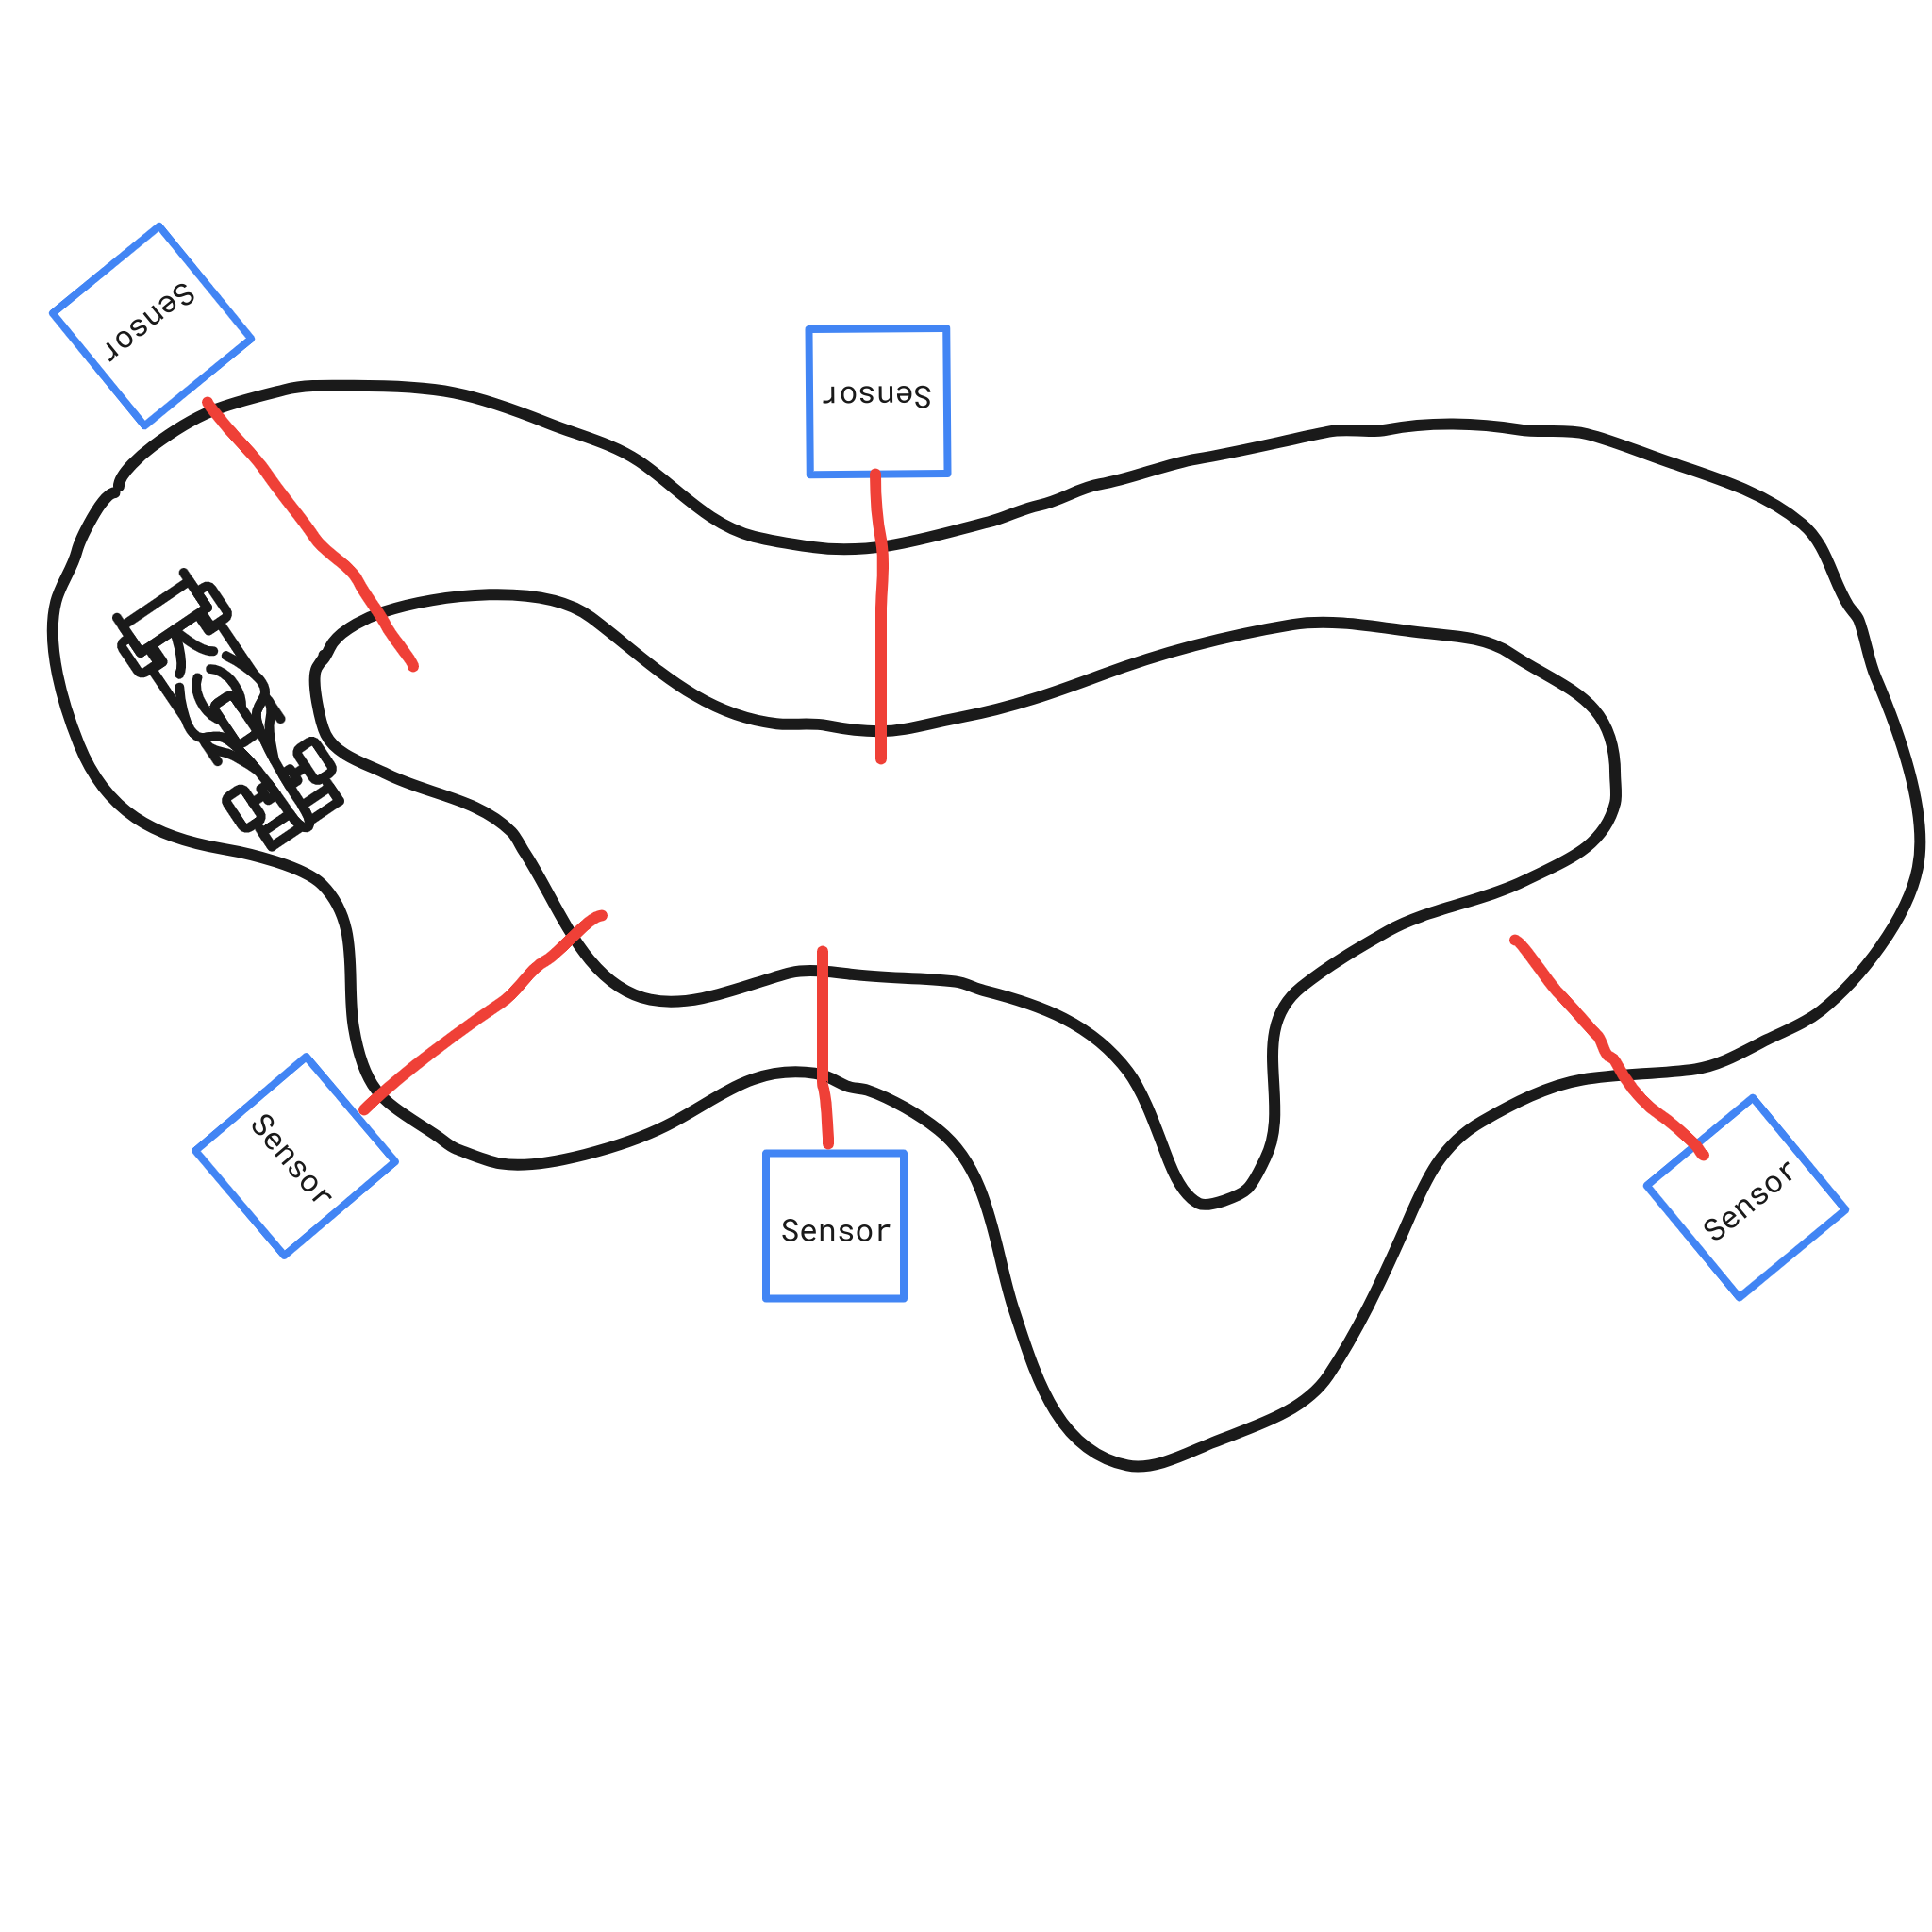
\includegraphics[width=\linewidth]{images/car_and_sensors.png}
    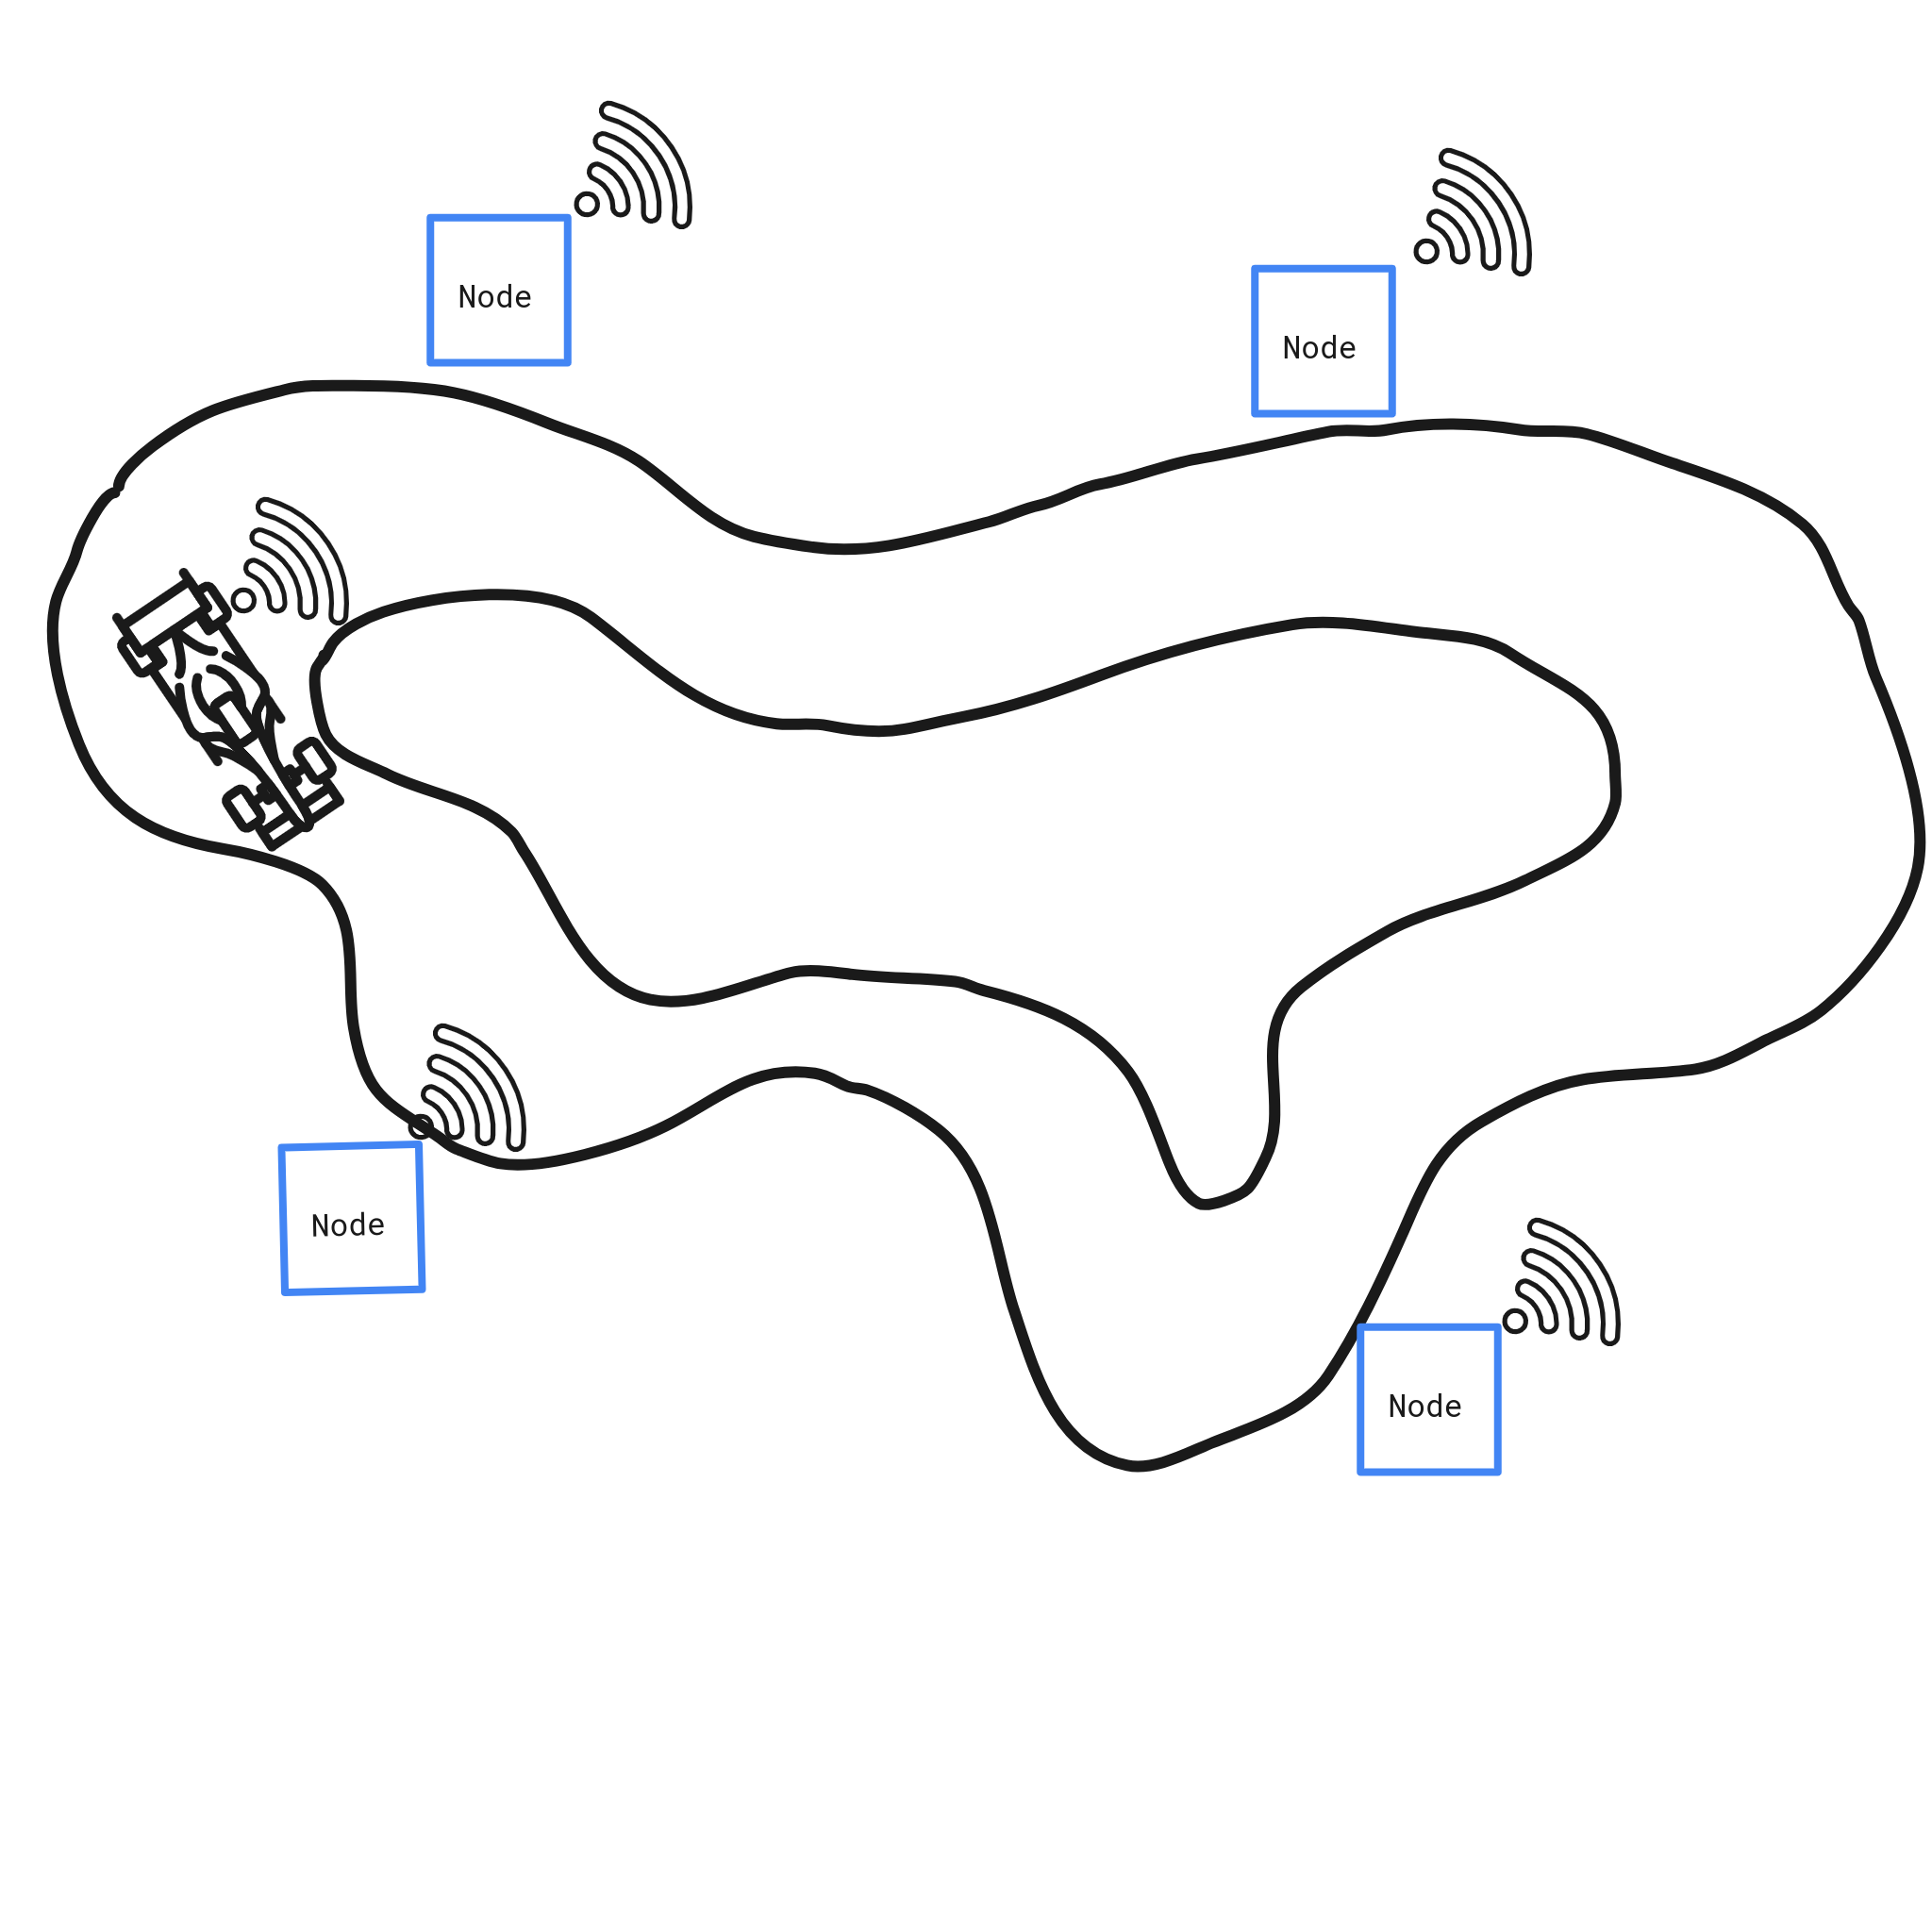
\includegraphics[width=\linewidth]{images/car_and_nodes.png}
    \caption{A visualisation of the physical similarities between a mesh network and sector timing system}
    \label{fig:node_sensor_compare}
\end{figure}

This sensor-mesh approach also conveniently handles part of our third goal, ergonomics. Mesh networks are, by definition, self organising. This means that they avoid many of the intricacies of setting up an AP for an end user since they can just be pre-configured by the creator. These mesh networks will also be more resilient to interference, since they can naturally route around something like a locally strong EMF. This should assist in abstracting away the complexities of networking from the user.

There is an issue with using a mesh network approach however. For either use case, an end user cannot get information out of the the network without also using a mesh compatible machine. This goes against our ergonomic goal. To solve this, we introduce a gateway node, which is simply a node that allows for access to the mesh network without participating in the mesh itself. End users will attach their computers to this node, allowing the mesh network to be abstracted away. To aid in 
debugging the mesh network from outside, a GUI will be developed that displays sensor node connection status.

\subsection{Components}
In summary, Timebay is comprised of:

\textbf{Sensor Nodes} - Nodes that handle both detection of a passing vehicle and organisation of the mesh network. Timebay should support 1-many sensor nodes in a network, where each sensor node is allocated a unique identifier. These nodes are fully wireless and battery powered to ease setup.

\textbf{Gateway Node} - A node that serves as the single entry point to the mesh, and Timebay as a whole. This node should have two network interfaces. One participates in the mesh, and the other allows for access to the mesh (via NAT, bridging or otherwise). Any centralised components of Timebay should also run on this server, such as network management utilities or databases.

\textbf{External Nodes} - Guests that participate in the mesh, but are not sensor nodes. These nodes use the mesh simply for its network access to the gateway or other external nodes. An example of an external node would be ISC's onboard PC.

\textbf{Clients} - End user computers that have no mesh compatibility. These are off the shelf laptops that may be running one of many OSes. Clients should connect to the external network interface on the gateway node to access all network resources. A cross-platform GUI application will be provided that will handle access to all of Timebay's timing functions.

\begin{figure}[t]
    \centering
    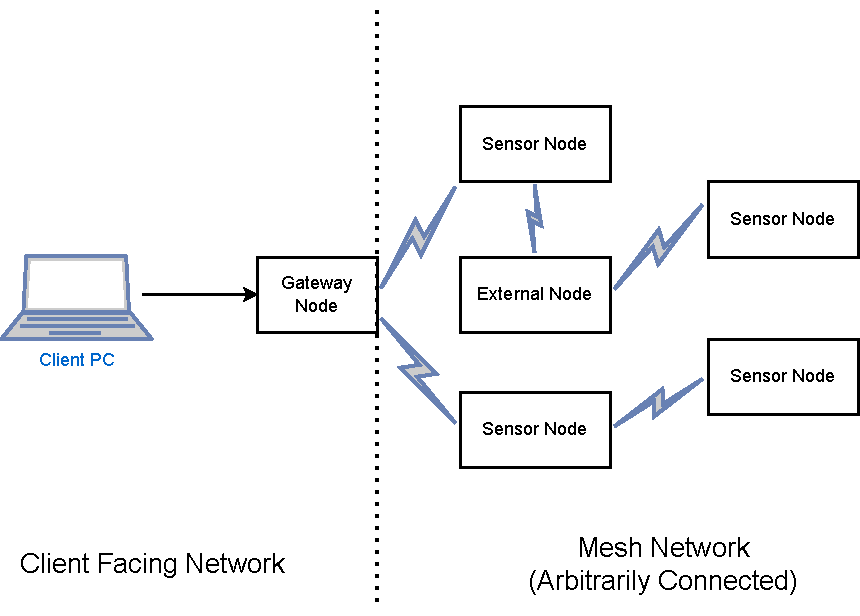
\includegraphics[width=\linewidth]{images/network_diag.drawio.pdf}
    \caption{High level network topology}
    \label{fig:high_level_net}
\end{figure}

\section{Implementation}

\subsection{Hardware}
\textbf{Nodes} - Our node implementation uses the Libre Compute Le Potato single board computer. This is a Raspi3 like board that has an 800Mhz processor, 2Gb RAM, and 1/100 Ethernet. To allow for wireless connectivity, we use ALFA AWUS036ACM (mt7612u chipset) wireless adapters.

\textbf{Sensor Nodes} - Vehicle detection will be preformed using a TF-Luna laser distance sensor. This sensor will be used like a line break sensor, detecting the vehicle when an object is detected some threshold closer than the zero point.

\textbf{Gateway Node} - Clients will connect to the gateway node using it's Ethernet port.

\begin{figure}[t]
    \centering
    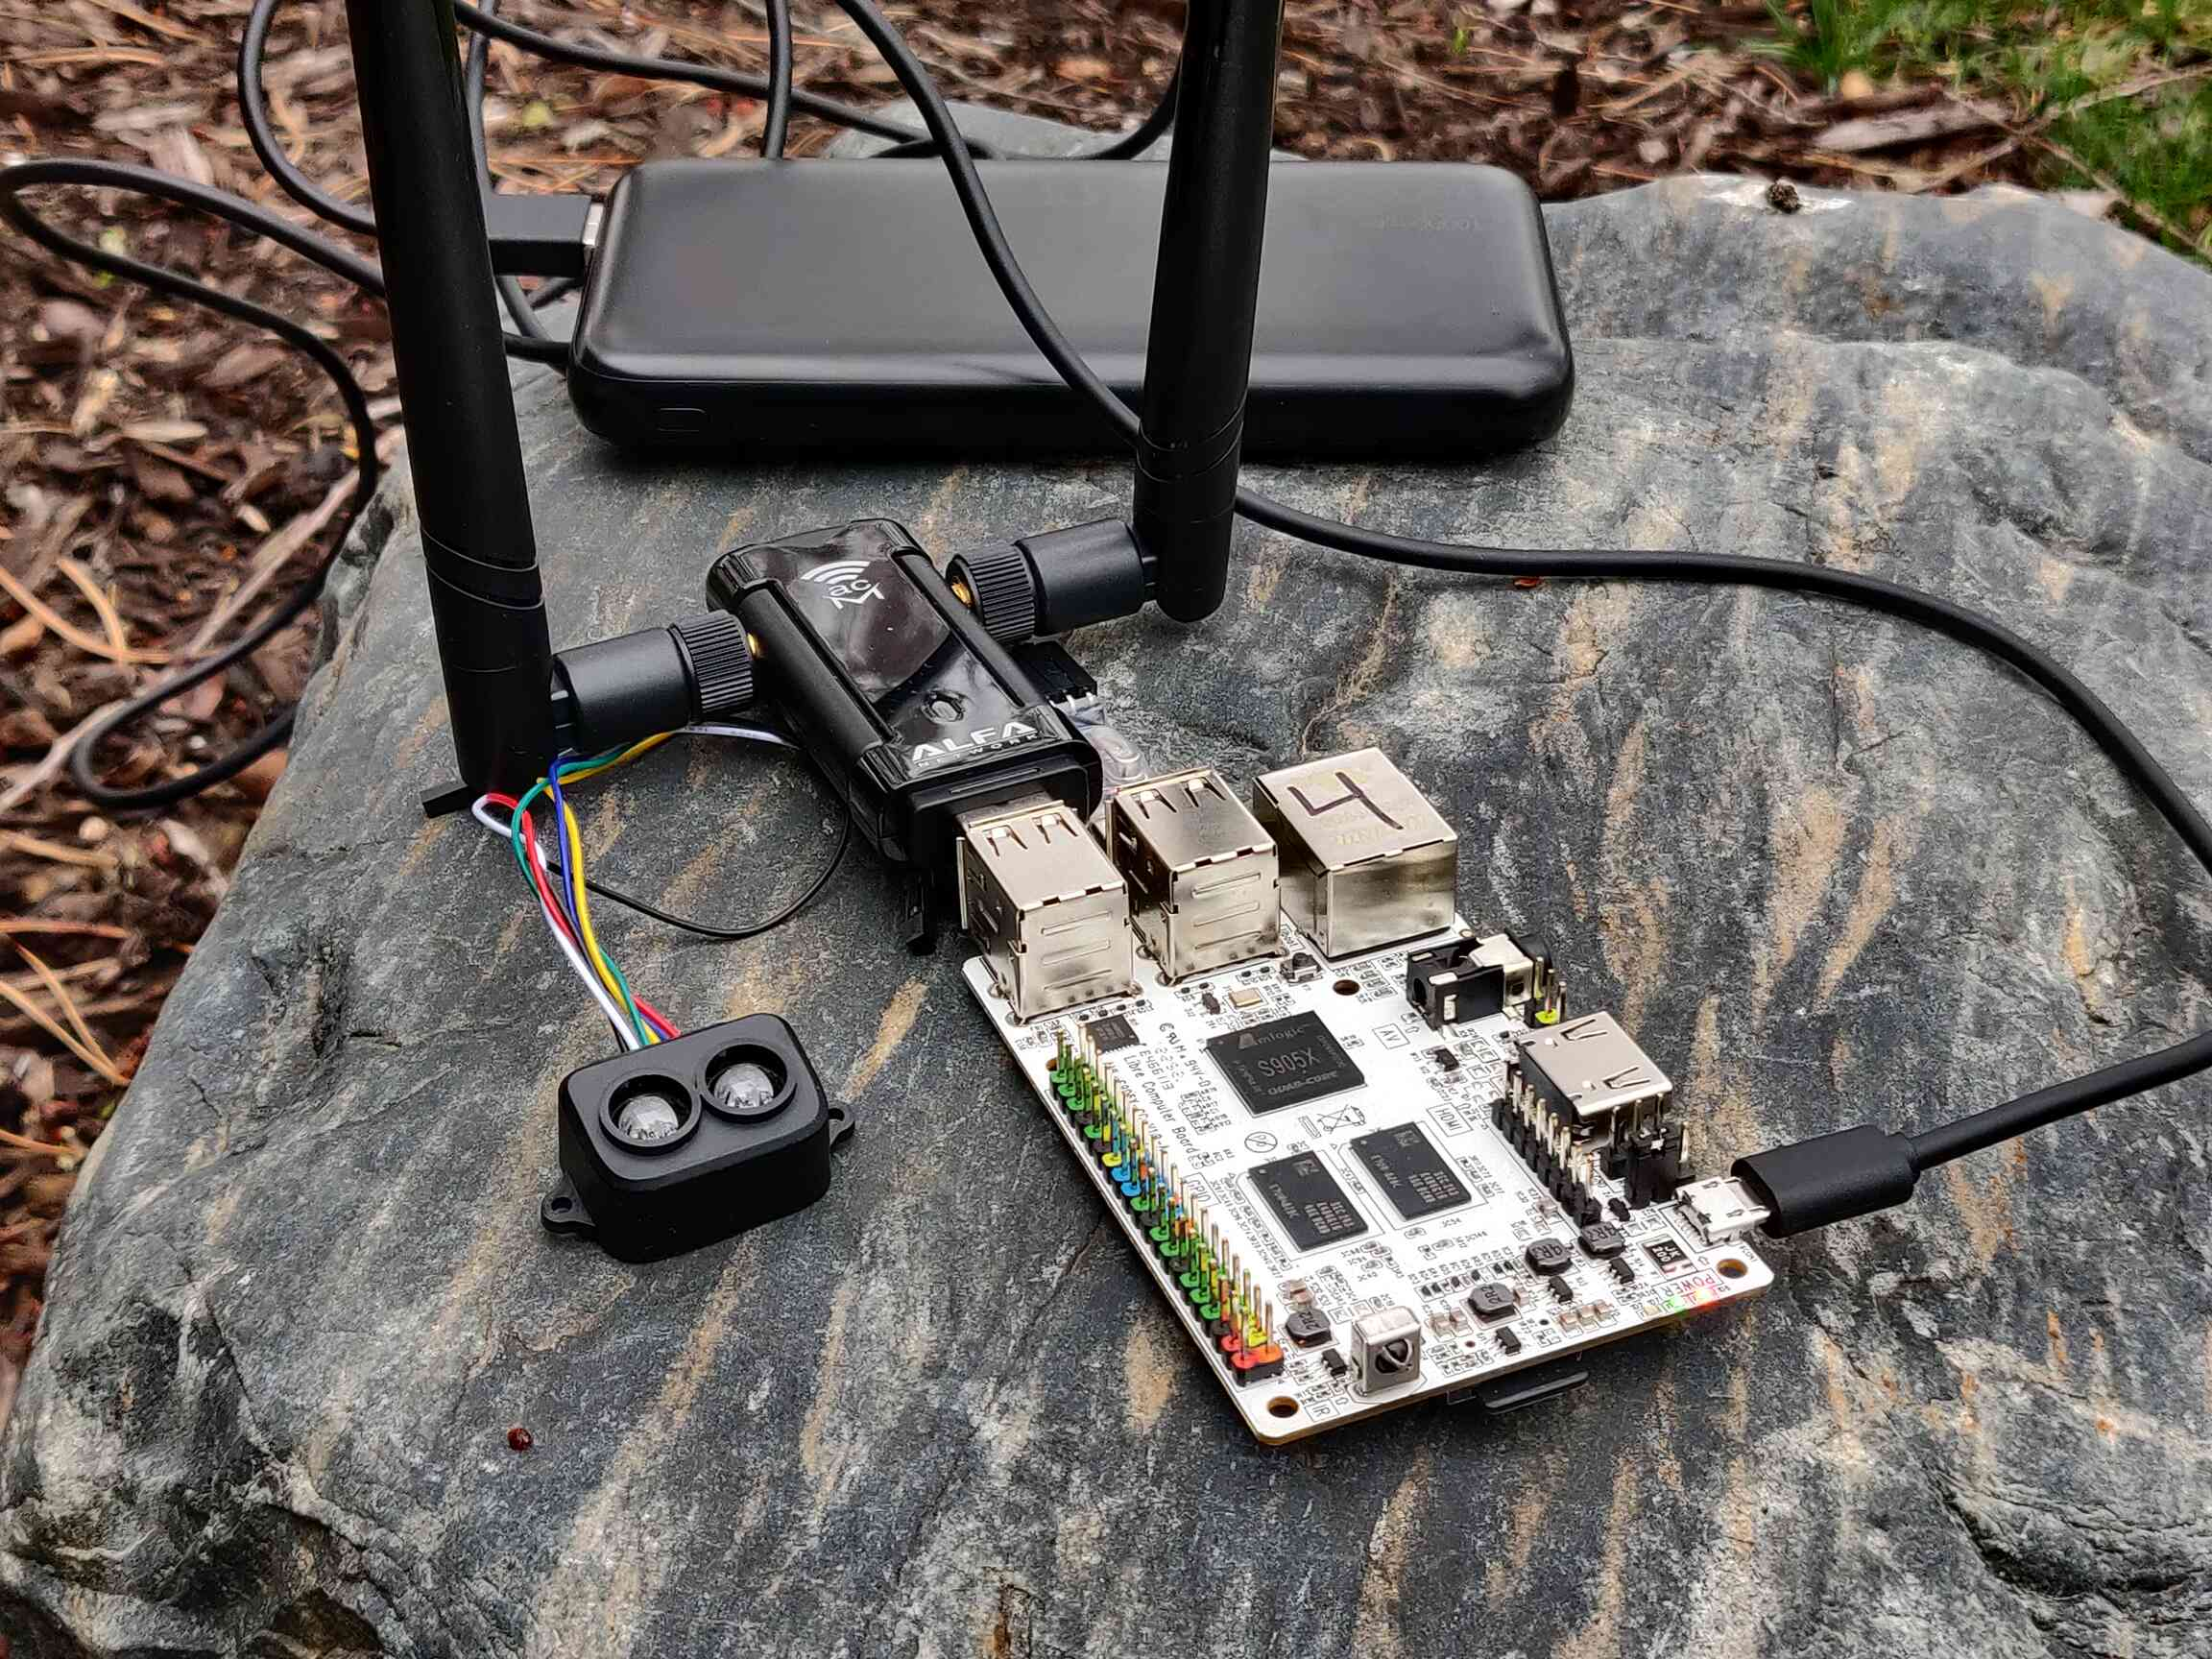
\includegraphics[width=\linewidth]{images/sensor_node.jpg}
    \caption{A sensor node}
    \label{fig:node}
\end{figure}


\subsection{Network}

The first key decision required for Timebays network implementation is a choice of physical layer protocol. Three main protocols were considered during this process.

\begin{itemize}
    \item \textbf{WiFi} - High bandwidth commodity standard
    \item \textbf{Bluetooth} - Low bandwidth, low power
    \item \textbf{Zigbee} - Lowest bandwidth, commonly used in mesh networks
\end{itemize}

Overall, Zigbee is likely the most fitting protocol, since it allows for using very low power devices for sensor nodes, and natively supports mesh networks. For Timebays use case however, Zigbee's middling 250Kbps bandwidth is simply too slow for some of the more intense activities ISC may perform \cite{haque_abdelgawad_yelamarthi_2022}. For example, creating an FPV video setup would require bandwidth well into the tens of megabits, which only WiFi supplies. For this reason, WiFi was chosen as the wireless protocol.

For our layer 2 mesh protocol, Timebay implements both a BATMAN-adv and 802.11s option. This is done due to the lack of conclusive evidence supporting either protocol as being definitively superior in the context of mobility. Additionally, little documentation exists regarding the current state of each project, or their associated hardware quirks.

All nodes get dynamic IPs in the 192.168.0.0/24 subnet, allocated by a DHCP server on the gateway node. The gateway node itself has the static IP 192.168.0.1, to allow for connections to centralized resources. DHCP was chosen over static IPs to allow for scaling the number of external nodes in mesh without requiring the user to maintain a record of allocated addresses.

To allow for clients to connect to the mesh network, the gateway node creates a Linux bridge interface between its Ethernet port and its mesh interface. The gateway node is only accessed via the IP address on the bridge, so clients connecting to the mesh can access any other mesh node as if they themselves were on the mesh. This also allows for clients to receive DHCP addresses, as DHCP will flow over the bridge. 

\subsection{BATMAN-adv Configuration}
BATMAN-adv is by default not very mobile friendly, as discussed in \cite{zeiger2009mobile}. Borrowing from that work, we will configure BATMAN to send OGM every 50ms. The goal of this is to minimize the time it takes for the mesh to reconfigure routes, critical to ensure dead nodes are routed around and mobile external nodes quickly change mesh links. To aid in this, OGM aggregation is also disabled, as recommended by the BATMAN-adv docs \cite{tweaking}. Both of these configurations will likely lower throughput, but should hopefully improve persistence in exchange. Following the results of \cite{8421863}, we will be using BATMAN IV over V.

\subsection{Sensor Node Communication}

All data related to the timing features of Timebay are broadcast across the network using MQTT. MQTT was chosen in this case not for its low bandwidth requirements (although this is nice), but rather its convenient pub-sub architecture which naturally mixes well with our highly dynamic network topology. The MQTT broker for Timebay is hosted on the gateway node.

The following topics are used:

\textbf{/connect} - Published to by nodes when they connect or reconnect to the broker. Nodes are allowed to publish to this topic when already connected, as a sort of heartbeat.

\textbf{/disconnect} - Published to by nodes when they disconnect from the broker, via LWT.

\textbf{/zero} - Causes all sensor nodes to zero their sensors.

\textbf{/sensors/detection} - Published to when a node detects a passing vehicle.

\begin{figure}[t]
    \centering
    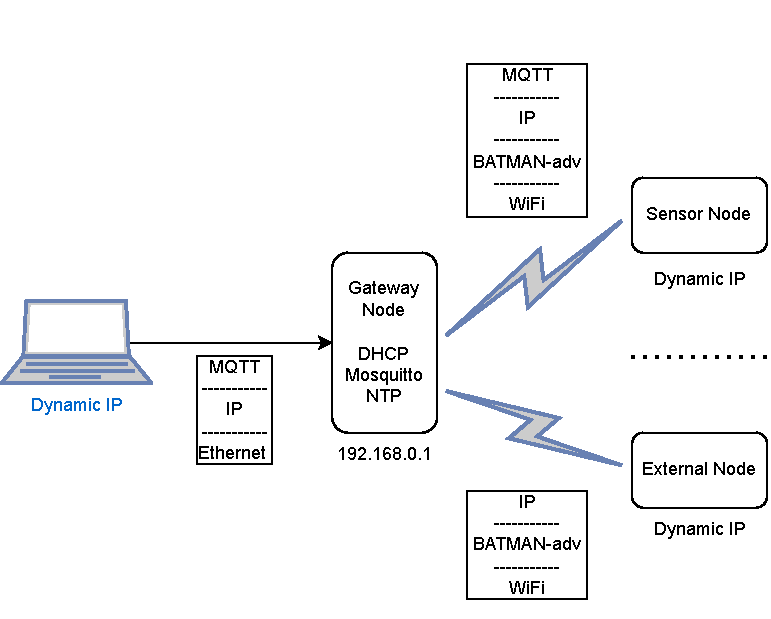
\includegraphics[width=\linewidth]{images/network_info.drawio.pdf}
    \caption{Timebay network implementation}
    \label{fig:network_impl}
\end{figure}
\subsection{Time}

As the name would suggest, time is rather important in Timebay. When sensor nodes send their data to the client to create sector times, we need to ensure that the client has an accurate estimation of the time that detection actually occurs. There are two ways to approach this problem:
\begin{enumerate}
    \item Timestamp when we receive sensor detections on the client
    \item Timestamp before we send the detection over MQTT, on the sensor node
\end{enumerate}
When evaluating this issue, it's important to remember that what we need to combat here is not the offset between the client and sensor nodes, but rather the \textit{offset} between each of the sensor nodes with respect to other sensor nodes. This is because lap times on the client are stored as absolute time values of the start and end of the sector. If one node's time has error from either approach, and that error is different than the error of any other node (what I call offset), the lap time will be inaccurate. 
From this view, it should be obvious that approach 1 is not viable. This is because every node on the network will naturally have different network latencies to the client, since synchronising latencies is not the goal of a mesh network. For approach 2, network latencies are not a direct issue. Instead, what adds offset is clock desyncronisation (or rather, clock offset as the term is normally used). Because the SBC's used for sensor nodes do not have a RTC, this necessitates the use of a clock synchronisation solution. 

Clock synchronisation in WSN is a well studied area \cite{9297296} \cite{elson2002fine} \cite{ping2003delay} \cite{maroti2004flooding}.
While these approaches do show promise, unfortunately few have open implementations, especially on Linux. Because we lack the resources to implement one of these protocols ourselves, we decide to simply use NTP, the traditional time synchronisation protocol on the Internet. As discussed in \cite{9297296}, an issue with NTP in mesh networks is the potential for asymmetrical latencies in RTTs. To help curb this issue, we chose Chrony as our NTP implementation. Chrony uniquely supports estimating delay asymmetry in its connections, going beyond the requirements of NTP itself \cite{RFC5905}.

Clock synchronisation in Timebay is implemented by synchronising all nodes to the gateway node, since that will be the node that is always present. Because we only care about reducing the offsets between sensor nodes, it does not matter that the gateway node itself may be desyncronised. Accordingly, Chrony is configured to use its local mode, which will serve NTP using the local clock as if it was synchronised. We also declare the servers stratum as 1, since we want all nodes to see the gateway as authoritative. Each sensor node runs Chrony configured to only access the gateway's server, forcing the clock to step if error is greater than 1 second. This is done in hope of forcing fast convergence on system setup, since all nodes will be greatly desynced on boot due to the lack of a RTC. 

\subsection{Sensor Node Detection}

The sensor node vehicle detection code is implemented as a Rust executable. Using the Tokio reactor, it polls over both an MQTT channel and the laser rangefinder concurrently, zeroing the sensor on MQTT command or sending a detection report to MQTT respectfully.

When detections have not occurred for some period of time (currently 3s), sensor nodes will send a heartbeat message on /connect. This is done not to tell if a node is disconnected, as MQTT does that with its own heartbeats, but rather to allow for late-joining clients to discover sensor nodes without requiring those nodes to have a detection.

\subsection{Deployment}

All Timebay nodes are implemented as Docker containers to help abstract over hardware heterogeneity, as well as to ease the difficulty of adding new sensor nodes. These containers are set up to boot on board restart via cronjob.

Because we need to access wireless interfaces from the container, we disable most virtualisation features of Docker. This involves running the container as privileged, using host networking, adding SYS\_TIME capability (required for NTP), and mounting /dev/.

To ease updating potentially many nodes, we set up a sort of 'OTA' update system. When a node boots, we configure its Ethernet port with DHCP if a carrier is available. In its bringup script, we fetch the Timebay repo's upstream. If we have a carrier on eth0 and the remote is ahead of HEAD, then we pull the remote and rebuild the docker container. This means that to update many nodes, one simply needs to plug them all into a switch and supply power.

The general boot process for sensor nodes is:
\begin{enumerate}
    \item Run bash script that git pulls Timebay, and rebuilds the docker container if new changes were pulled
    \item Run docker container
    \item Find a mesh/IBSS compatible interface by scraping iw output
    \item Use iw to set the device to IBSS/Mesh mode
    \item If using BATMAN-adv, setup bat0 interface
    \item Start dhcpcd to get IP address
    \item Start sensor node executable
\end{enumerate}

\subsection{GUI}

The client GUI application is also implemented in Rust, and utilises shared components with the sensor node. The GUI implements all of the actual application logic for sector timing, aggregating data collected from the MQTT broker. Sectors are defined by pairs of nodes starting at the lowest node id and pairing until the last node, which is paired with the initial node id. Each sector begins timing at the end trigger of the last sector, updating the GUI as the course is completed. 

If the car skips a node, the time spent in the sector is simply rolled into the next sector, and the skipped sector is marked invalid. This transparently handles nodes disconnecting, since they will simply be skipped. The alternative would be to invalidate the sector eagerly when the node disconnects but before the car passes it, but this idea was discarded as it complicates the logic of the node coming back online. By treating disconnected nodes as if they were skipped, we optimistically give the node a chance to reconnect with the network without any sort of special logic.

Should the nodes clocks become desynced, it is possible for the GUI to detect the detection timestamps going back in time. If this occurs, the current sector is marked as invalid. 

When a lap is completed, the GUI calculates the complete lap time and moves the splits to one side of the screen, and then displays the time deltas with respect to the prior lap.

Also included in the GUI is a display of all currently connected nodes, as well as a button to zero the sensors. Nodes will display as connected as soon as they send a message to /connect, and will show as disconnected 10 seconds after disconnecting, since we have configured a 10s TTL.

In an attempt to make this GUI as cross platform as possible, it is actually implemented in the terminal, making it a TUI. This avoids linking with platform specific GUI libraries, increasing the chance of the GUI remaining compatible on future, unknown OS versions.


\begin{figure}[t]
    \centering
    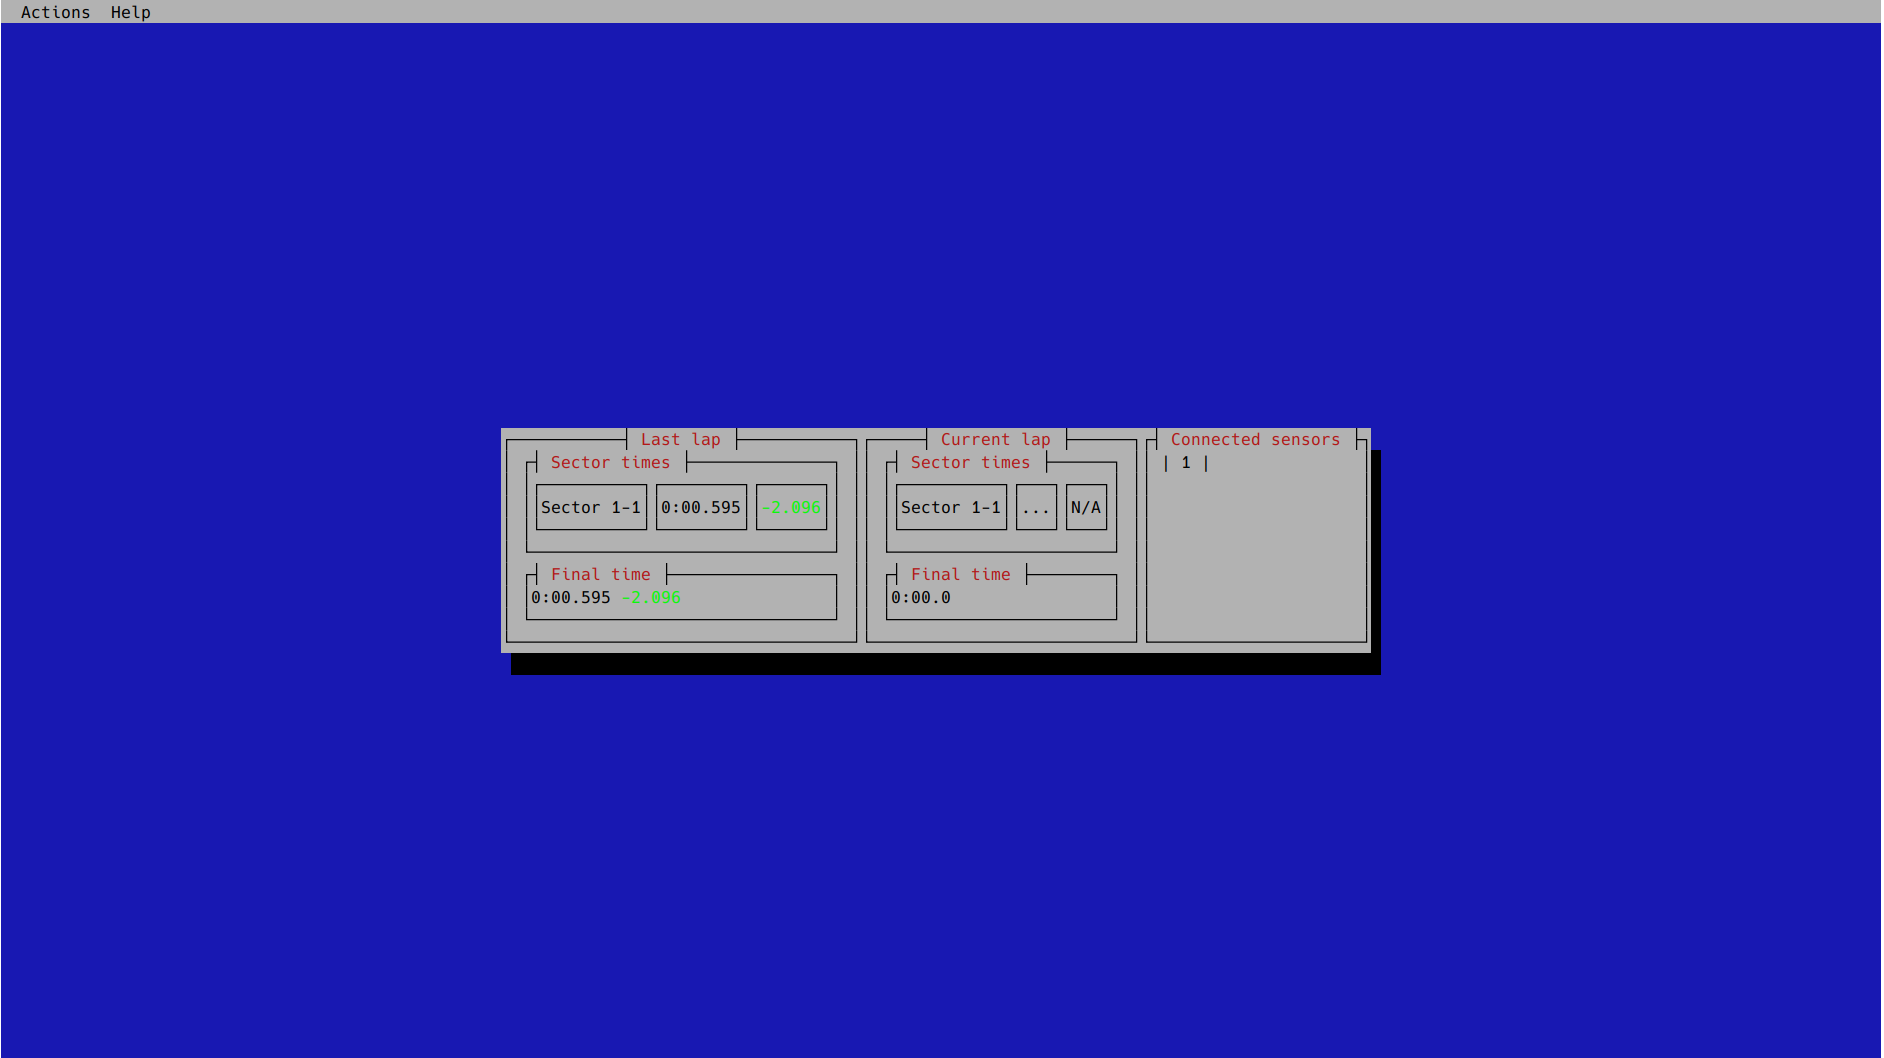
\includegraphics[width=\linewidth]{images/gui.png}
    \caption{Timebay's GUI connected to a single sensor node}
    \label{fig:gui}
\end{figure}

\subsection{Ergonomics}

Timebay's third goal, ergonomics, is primarily achieved by designing the network to be as self operational as possible. For example, all mesh networking is abstracted away by the gateway node. If a node disconnects, one simply needs to wait for it to re-mesh, since the GUI will automatically handle how that addition or reduction of a node will impact lap times. If the layout must be changed, all the user must do is press the zero sensors button in the GUI and the system will be operational again. Mobile batteries are used to power the nodes as opposed to LiPos to allow for easy recharging of nodes by non electrical members.

In addition to these and many more design choices, we make a point to supply ample documentation of the system. This is important, since the student teams have very high turnover, and organisational knowledge around tools is very volatile. In particular, instructions to replicate the current implementation are provided, as well instructions for operation, troubleshooting, and development. To ensure these are not lost while the hardware remains in use, Timebay is open sourced via a GitHub repository\footnote{https://github.com/andyblarblar/timebay}.

\section{Evaluation}

\subsection{Startup time}
First, we will evaluate the startup time in optimal conditions. To measure this, we set up three sensor nodes in a 3m circle around the gateway node attached to a client. A timer is started on the computer, then all nodes are turned on. With the GUI open, we wait until all nodes are displayed in the connected nodes table. The results are shown in Fig. \ref{tab:startup}. Note that this includes the time for:
\begin{enumerate}
    \item Booting Linux
    \item Starting Docker
    \item Connecting to mesh
    \item Getting IP over DHCP
    \item Connecting to MQTT
\end{enumerate}
The average startup time was 3:51 for BATMAN, and 3:20 for 802.11s. Upon investigating the boot logs, it appears that approximately 2:40 of this boot time is spent booting the host OS. This is likely due to a misconfigured service. Because both protocols use the same Docker container, the consistently faster boot times on 802.11s is likely due to properties of its mesh. In particular, DHCP is a likely candidate for this lost time. As we will see later, BATMAN-adv has very large packet loss. DHCP requests addresses using a UDP broadcast. Given this best effort approach, dhcpcd's exponential back-off on failure, and the large packet loss, DHCP can take quite a while to gain an address in BATMAN-adv meshes. This was verified by Wireshark analysis, where DHCP requests could be seen leaving the node but not receiving a response. This could also explain the greater variance shown in the BATMAN-adv results.

\begin{figure}[t]
\begin{tabular}{|l|l|}
\hline
\textbf{Trial (BATMAN-adv)} & \textbf{Time Till complete} \\ \hline
1              & 3:30                        \\ \hline
2              & 3:55                        \\ \hline
3              & 3:44                        \\ \hline
4              & 4:21                        \\ \hline
5              & 3:44                        \\ \hline
\end{tabular}

\begin{tabular}{|l|l|}
\hline
\textbf{Trial (802.11s)} & \textbf{Time Till complete} \\ \hline
1              & 3:11                        \\ \hline
2              & 3:20                        \\ \hline
3              & 3:25                        \\ \hline
4              & 3:20                        \\ \hline
5              & 3:24                        \\ \hline
\end{tabular}
\caption{Timebay startup times}
\label{tab:startup}
\end{figure}

\subsection{Clock Synchronisation}
Next, we will verify that nodes are being synchronised. This test can be seen as a validation of goal 1, since the sector timing logic works as expected, leaving only the clock synchronisation as a potential issue. This is done by placing two sensor nodes next to one another, then dropping a piece of cardboard in front of them. Because the nodes should trigger at roughly the same time, we can compare the GUI's received timestamps to find the offset of the clocks, and thus the error our timing system will see per sector. This process is begun first by rebooting the nodes to force a fresh NTP state, then collecting five samples when the nodes appear in the GUI. The results of this experiment are displayed in fig. \ref{tab:times}. Note that stamps include only the nanoseconds component, as no readings had greater than a second of error. Offsets are rounded to the ms as our testing apparatus does not have ns accuracy. 

These results show us a few things. First, our aggressive stepping of clocks until second accuracy is achieved has achieved its goal of getting the clocks reasonably synchronised within a short period of time. Second, even with very little time to converge, both protocols have an acceptable level of error. 802.11s especially, with all measurements under 10ms. While this advantage could be from NTP having issues contending with BATMAN's packet loss, our testing apparatus has too much potential for procedural error for this to be conclusive.

\begin{figure}[t]
\begin{tabular}{|l|l|l|l|}
\hline
\textbf{BAT} & \textbf{Node 1 stamp} & \textbf{Node 2 stamp} & \textbf{Offset} \\ \hline
1              & 133668199ns           & 158070397ns           & 24ms            \\ \hline
2              & 568918805ns           & 570767970ns           & 2ms             \\ \hline
3              & 728301891ns           & 746114176ns           & 18ms            \\ \hline
4              & 503307445ns           & 501268735ns           & 2ms             \\ \hline
5              & 331404650ns           & 335236888ns           & 4ms             \\ \hline
\end{tabular}

\begin{tabular}{|l|l|l|l|}
\hline
\textbf{802.11s} & \textbf{Node 1 stamp} & \textbf{Node 2 stamp} & \textbf{Offset} \\ \hline
1              & 710317045ns           & 758237086ns           & 8ms            \\ \hline
2              & 321956813ns           & 334979791ns           & 1ms             \\ \hline
3              & 409371012ns           & 430514388ns           & 2ms            \\ \hline
4              & 328401762ns           & 355385103ns           & 3ms             \\ \hline
5              & 716304263ns           & 731996424ns           & 2ms             \\ \hline
\end{tabular}
\caption{Timebay clock synchronisation offsets}
\label{tab:times}
\end{figure}

\subsection{Packet Loss}
While performing other tests, many were failing to pass due to massive packet loss. To investigate this issue further, we test the packet loss under various setups to find any patterns. For all of these configurations, the client is connected to the gateway node and SSHs into it. From the gateway node, we use ubuntu's ping utility to test the packet loss to one of the sensor nodes until 150 sequences are reported. For each configuration, we repeat this test for 1, 2, and 3 connected sensor nodes. The results of these tests are shown in fig. \ref{fig:packetloss}.

First, we test BATMAN-adv with 50ms OGM, which was the configuration initially proposed. As shown in fig. \ref{fig:packetloss}, there is a massive jump in packet loss when a second node is added, with a further increase with a third. To investigate if this issue was caused by our aggressive OGM rate, we run the test again with 500ms OGMs. Once again, packet loss jumps massively when a second and then third node are added, although less so than with the 50ms OGM. To ensure this isn't a fundamental issue with our system, we finally repeat the test with 802.11s. These results are a little hard to view in the chart, since there is \textit{literally no} packet loss, regardless of node count. This result was quite surprising, since other literature on BATMAN-adv does not document packet loss issues. The packet loss only begins once IP data begins to be sent, not when the IBSS forms. Because of this, its possible this is a misconfiguration of BATMAN-adv, although we use all default settings aside from OGM rate, which makes this unlikely.

\begin{figure}[t]
    \centering
    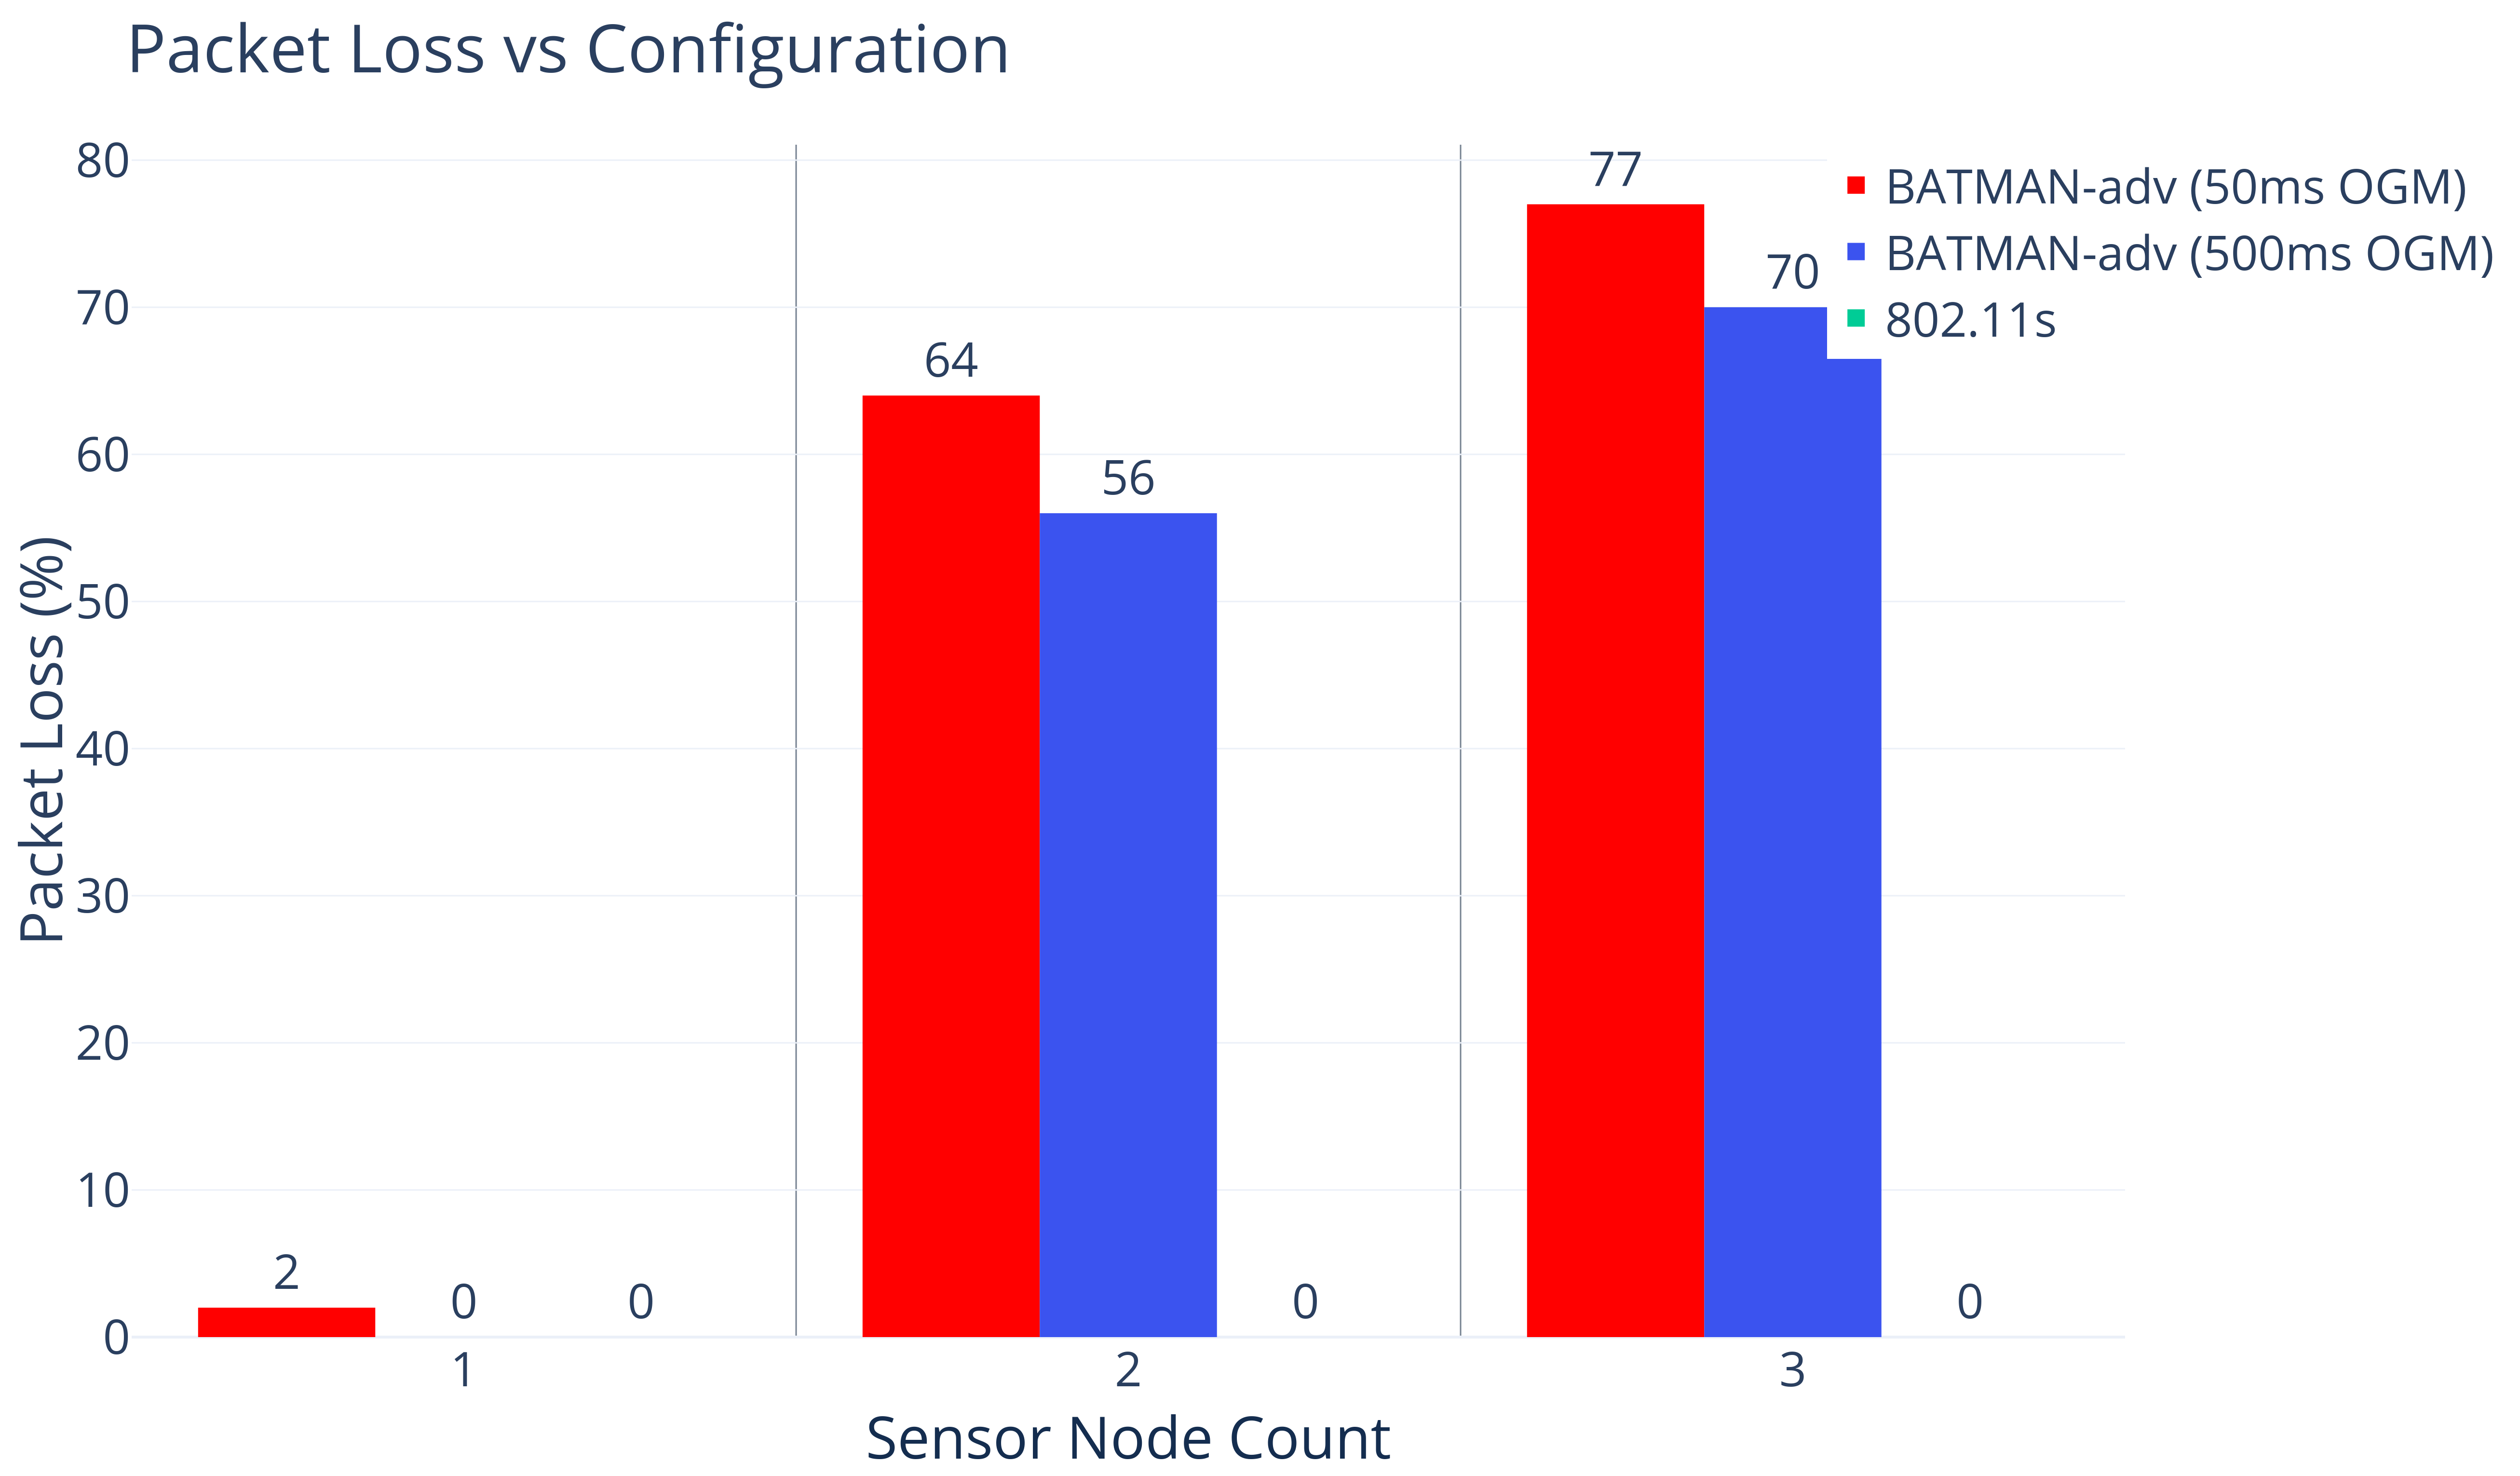
\includegraphics[width=\linewidth]{images/Packet Loss vs Configuration.png}
    \caption{Packet loss under various configurations}
    \label{fig:packetloss}
\end{figure}

\subsection{Throughput In Motion}

\begin{figure}[t]
    \centering
    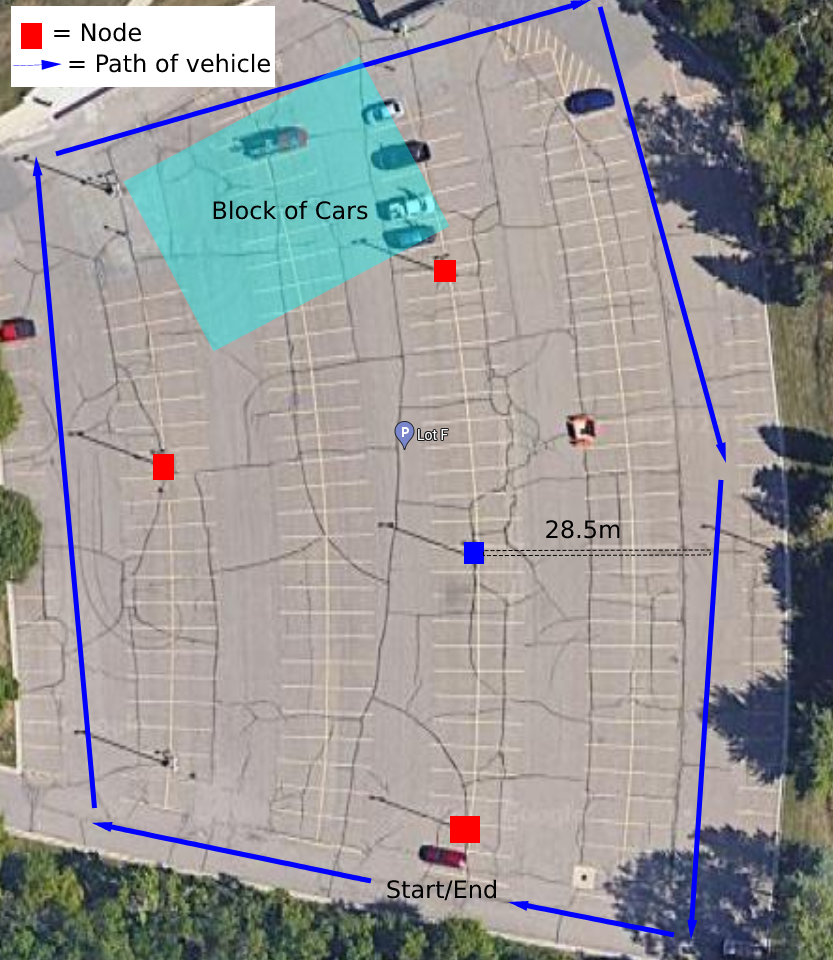
\includegraphics[width=\linewidth]{images/testing_lot.png}
    \caption{Testing setup for throughput tests}
    \label{fig:lot}
\end{figure}

Finally, we will evaluate throughput of the mesh with a vehicle in motion. This can be seen as a validation of goal 2. Unfortunately, neither teams vehicle was available for testing. As a stand in, a collaborator's \textit{2023 Ford Maverick XLT 2.0L EcoBoost AWD} will serve as our vehicle. To ensure fair results, we have a laptop held in the bed of the truck to prevent the body from blocking signals. This is important because both student vehicles allow for unobstructed antennas. Testing was done on a parking lot on campus, with 3 sensor nodes and the gateway node spread throughout. The distribution of these nodes is displayed in fig. \ref{fig:lot}. The laptop held in the bed will be simulating the onboard PC of ISC, connected to the mesh as an external node. We will only perform these tests using 802.11s, since BATMAN-adv's packet loss was too high to perform the test with 5 total nodes. For each test, the vehicle will drive the perimeter of the lot while iperf3 runs a TCP bandwidth test of the network between a client connected to the gateway and the external node on the vehicle. Pings will run for all tests to collect aggregate latency measurements. The results of these tests can be seen in fig. \ref{fig:throughput}.

\begin{figure*}[t]
    \centering
    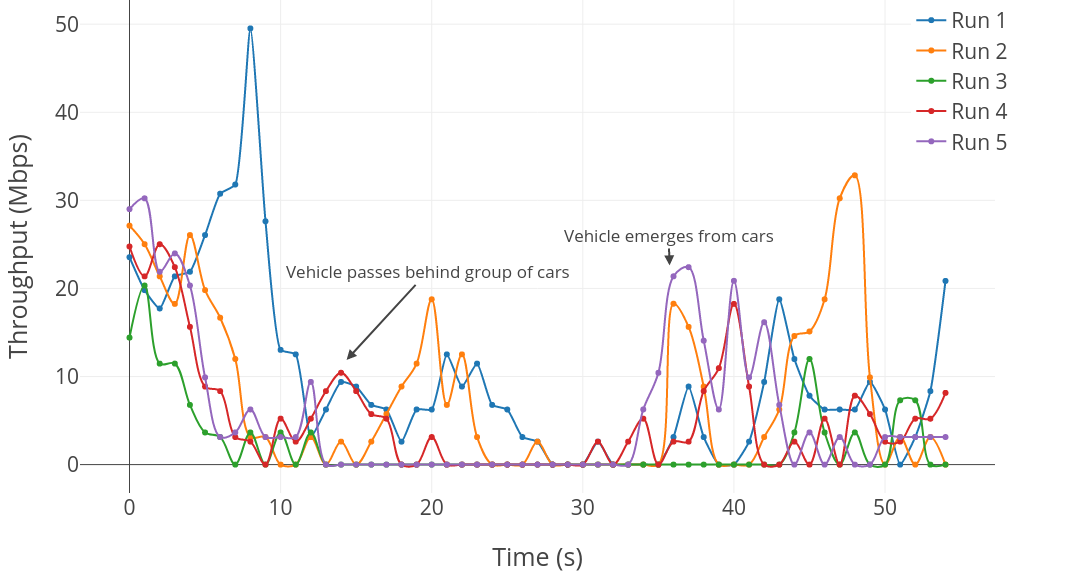
\includegraphics[width=\linewidth]{images/throughput.png}
    \caption{Throughput of the mesh with vehicle in motion}
    \label{fig:throughput}
\end{figure*}

As can be easily observed, Timebay has very large amounts of jitter while in motion. This was not unexpected, and tracks with the results of \cite{8417706}. This can be seen in the latency results, where we see a minimum RTT of 1.3ms, a max of 1800ms, an average of 68ms, and a standard deviation of 123ms. From the period of around 15s - 34s, a large drop in throughput, or even the connection, can be seen in all runs. This is due to a large block of parked cars in the lot fully obscuring the vehicle from all nodes. This gives us the opportunity to observe the mesh reforming under motion, which it does very smoothly shortly after the vehicle emerges at approx. 35s. Note that because of this, 35s onwards is the most representative of an average use case, as the vehicle is in motion and in range of at least one node. This range still shows large variance in throughput, ranging from 2Mbps to 20Mbps depending on the run. Overall, these results show that Timebay is not suitable for real time data transfer from an external node, such as for teleoperation. It is, however, capable of transferring data at reasonable speeds (faster than alternative wireless standards) in jitter durable applications. An example of this could be viewing ROS topics from the external node in Rviz, where latency is less of a concern than persistence and reasonably fast speeds.

It is worth pointing out that the above results apply to a vehicle in motion only. While stationary, Timebay can maintain consistently high speeds, sometimes even pushing up against the bandwidth of the 1/100 gateway link. This applies to both the vehicle while stationary, as well as other possible uses of external nodes, such as remote terminals around the circuit.

\subsection{BATMAN-adv vs. 802.11s}
As can be seen throughout the evaluation, the choice of BATMAN-adv vs. 802.11s significantly changes the behavior of Timebay. Of course, Timebay can only use one of these protocols at a time, so it is worthwhile defining a default.

A running theme throughout the creation of Timebay was the mesh protocols acting significantly differently given different hardware. Initially, the system used wireless adapters in the rt2800 chip-set family. While using these drivers, 802.11s was unable to bridge with the Ethernet port on the gateway, preventing the use of 802.11s in Timebay. When the project moved to adapters that used the Linux mt7x drivers for unrelated reasons, 802.11s was fully operational. This poses a significant issue for recommending a protocol, since reproductions of Timebay in the future may outright not function if chip-sets change even in vetted adapters. Unfortunately, BATMAN-adv was nearly unusable with multiple nodes in either setup due to its massive packet loss. However, it was capable of bridging even with the rt2800 adapter. Awkwardly, this leaves BATMAN-adv with a niche where it is still technically better than 802.11s, by virtue of running at all.

Overall then, 802.11s is currently far and away the better implemented protocol on Linux, so long as you have an adapter with the correct chip-set. If you don't, then BATMAN-adv can be used as a fallback, although it shouldn't be used with more than one sensor node.

\section{Conclusion}

\subsection{Limitations}

\subsubsection{Security}
Timebay lacks any security whatsoever. This means that anyone is capable of connecting to the mesh and accessing its resources. Realistically, this primarily makes external nodes like ISC's PC vulnerable to external connections if not secured. For a more professional application, this would also make the system vulnerable to passive and active attacks on the sensor detection times over MQTT. This could be an issue if say, a formula team is practicing around competitors. For the intended use case, I do not consider this a large issue, since the onboard PC is already secured and messing with lap times is harmless. The system should be amendable to hardening many of its interfaces, such as requiring a password for MQTT and encrypting WiFi using 802.11s's SAE \cite{en:developers:documentation:ieee80211:802.11s}.

\subsubsection{SBCs}
Timebay, by its reliance on Linux, requires the use of SBCs that are likely far more powerful than needed. This reliance comes from a few sources:
\begin{enumerate}
    \item Mesh Implimentations
    \item Current sensor node implementation codebase
    \item NTP
\end{enumerate}
While 2 could be programmed away, 1 and 3 are far more difficult. Both mesh algorithms and clock synchronisation suffer from a lot of theoretical algorithms but a lack of implementations. Even when implementations are available, they are often for a particular embedded OS, lowering the odds of the other system also being available. Should this issue be resolved, Timebay could likely be implemented using a micro-controller like the ESP32 as the sensor node platform, although throughput would need to be re-verified.

\subsection{Future Work}
Timebay is still a very young system, and has many areas that could be significantly improved given future work. 

\subsubsection{802.11s Parameters}
All tests were performed using default 802.11s parameters, largely due to a lack of time for iteration. These parameters, especially those controlling the HWMP, can likely be significantly optimised for the moving vehicle scenario. 802.11s also natively supports the concept of gateway nodes, something that we do not utilise in this work.

\subsection{WiFi}
All mesh configurations currently use 2.4ghz channel 5 with HT40+ for their underlying WiFi connections. Channel 5 was chosen after a site survey of campus found it to be the least congested. Even with this choice, the 2.4ghz spectrum is very polluted from various industrial machines around campus. Future work should investigate both the use of the 5ghz spectrum as well as various channel widths to potentially increase throughput and other metrics.

\subsubsection{Hardware}
To improve ergonomics, Timebay could greatly benefit from standardised boxes for the nodes. This would improve setup times, lower the chance of environmental damage, and overall improve ease of use. These should be able to be constructed with 3d printers, allowing us to open source the design alongside the codebase.

\subsection{Summary}
To aid two student teams at the University of Michigan Dearborn, we analyse some shared deficiencies between the teams. This uncovered the need for both a granular timing system, and a large-scale network for vehicle connections. To solve both issues together, we combine the existing solutions of sector timing and mesh networking into one system, called Timebay. Upon evaluation, Timebay is shown to excellently fulfill its timing duties, with only a 3.2ms average error per sector using 802.11s. The mesh network is shown to provide network access to the vehicle while still and within the range of a node, but suffers from jitter in throughput and latency while in motion. Overall, Timebay should adequately address the needs of UMD-Racing, and greatly improve the networking conditions of ISC. Future work should focus on improving network conditions while the vehicle is in motion, potentially opening up new avenues of use for Timebay within ISC.

% Can use something like this to put references on a page
% by themselves when using endfloat and the captionsoff option.
\ifCLASSOPTIONcaptionsoff
  \newpage
\fi

\bibliographystyle{IEEEtran}
\bibliography{bibtex/bib/timebay}

% that's all folks
\end{document}


